\documentclass[xcolor=table]{beamer}
\usepackage[utf8]{inputenc}
\usepackage[T1]{fontenc}
\usepackage[alf]{abntex2cite}
\usepackage{udesc}
\usepackage{amsfonts,amsmath,amssymb,mathtools}
\usepackage{verbatim}
\usepackage{listings}
\usepackage[ddmmyyyy]{datetime}
\usepackage{hyperref, url}
\usepackage{graphicx}
\usepackage{bussproofs}
\usepackage{multirow}
\usepackage{changepage}

\usepackage{svg}
\setsvg{inkscapeexe=inkscape}
\setsvg{inkscapeopt=-z -D}

\newcommand{\uglyphi}{\phi} % mantendo o \phi velho
\renewcommand \phi{\varphi}
\let \emptyset \varnothing

\newcommand{\Ltac}{$\mathcal{L}$\unskip tac}

\graphicspath{{Figuras/}}
\setbeamertemplate{frametitle continuation}{}

% suprimindo warnings do hyperref
\pdfstringdefDisableCommands{%
  \def\\{}%
  \def\texttt#1{<#1>}%
  \def\smallskip{}%
  \def\medskip{}%
}

\renewcommand{\figurename}{Figura}
\renewcommand{\tablename}{Tabela}
\sloppy
\title[]{Formalização e Prova de algoritmos de menor caminho usando Coq}

\author[João Vitor Fr\"ohlich]{
    João Vitor Fr\"ohlich\\\smallskip
    {\scriptsize Universidade do Estado de Santa Catarina \\\smallskip
    \vspace{-2mm}
    \texttt{joaovitorfrohlich@gmail.com}\\\medskip
    {Orientadora: Dra Karina Girardi Roggia}\\
    }
}

\date{\today}

\titlegraphic{Apoio:\\
\includegraphics[scale=.15,keepaspectratio]{Logo-CNPq.png}}
\logo{
\includegraphics[scale=.05,keepaspectratio]{Logo-Função.png}}

\begin{document}

    \begin{frame}
        \titlepage
    \end{frame}

    \begin{frame}[allowframebreaks]{Sumário}
        \tableofcontents
    \end{frame}

    \section[]{Introdução}
    \begin{frame}{Introdução}
    \begin{itemize}
        \item Formalização e Prova
        \begin{itemize}
            \item [--] Especificação Formal
        \end{itemize}
        \item Algoritmos de menor caminho
        \begin{itemize}
            \item [--] Teoria de Grafos
        \end{itemize}
        \item Coq
        \begin{itemize}
            \item [--] Assistentes de Provas
        \end{itemize}
    \end{itemize}
\end{frame}
    % \begin{frame}{Introdução}
    \begin{itemize}
        \item Linguagens modais são uma excelente ferramenta para raciocinar sobre estruturas relacionais - conjunto base e relação(ões) sobre este conjunto.~\cite{blackburn2001modal}.
        \item Não é difícil imaginar situações onde possa ser relevante um sistema lógico que contenha diversas modalidades interpretadas de maneira diferente;
        \item Para obter estes sistemas lógicos, pode-se utilizar do método da fusão de lógicas modais, que permite combinar diversos sistemas de lógica modal em um único sistema.
    \end{itemize}
\end{frame}
    % \begin{frame}{Introdução}
    \begin{itemize}
        \item Assistentes de provas são softwares para desenvolvimento de provas formais;
        \item Coq é um assistente de provas com grande disponibilidade de materiais didáticos e diversas ferramentas que facilitam no desenvolvimento de provas~\cite{silva2019certificacao};
        \item Fusões de lógicas é um tópico complexo, porém as dificuldade referentes à isso podem ser amenizadas com o uso de assistentes de provas como o Coq.
        \item Continuação do que foi desenvolvido em~\cite{silveira2020implementacao} e~\cite{silveira2022sound}.
    \end{itemize}
\end{frame}

    \section[]{Objetivos}
    \begin{frame}{Objetivo Geral}
    O objetivo geral deste trabalho é formalizar e provar em Coq algoritmos de busca do menor caminho entre dois pontos em grafos.
\end{frame}
    \begin{frame}{Objetivos Específicos}
    \begin{enumerate}
        \item Estudar os principais algoritmos determinísticos de busca do menor caminho de grafos
        \item Estudar os principais algoritmos heurísticos de busca do menor caminho em grafos
        \item Implementar alguns algoritmos de busca do menor caminho em assistente de provas, que serão escolhidos de acordo com critérios a serem estabelecidos
        \item Provar a corretude da implementação dos algoritmos definidos
    \end{enumerate}
\end{frame}

    % \section[]{Trabalhos Relacionados}
    % \begin{frame}{Trabalhos Relacionados}
    \begin{enumerate}
        \item \citeauthoronline{benzmuller2010combining} (\citeyear{benzmuller2010combining}) -
            apresenta fusões de lógicas modais em Cálculo-\(\lambda\) Simplesmente Tipado e modelagem de lógicas combinadas em diversos assistentes de provas;
        \item \citeauthoronline{fuenmayor2019mechanised} (\citeyear{fuenmayor2019mechanised}) -
            descrevem lógicas modais resultantes de combinação em Isabelle;
        \item \citeauthoronline{lescanne2007dynamic} (\citeyear{lescanne2007dynamic}) -
            descrevem uma lógica modal resultante de fusão em Coq;
        \item \citeauthoronline{rabe2017identify} (\citeyear{rabe2017identify}) -
            modela sistemas lógicos e combinações de lógicas em uma linguagem baseada em teoria de tipos chamada M\textsubscript{MT}.
    \end{enumerate}
\end{frame}

    \section[]{Teoria de Grafos}
    \begin{frame}{Definições - Grafo direcionado}
    \begin{itemize}
        \item $G = \langle V,E,\delta_0, \delta_1 \rangle$;
        \begin{itemize}
            \item[--] Restrição de laço: $\forall e \in E, \delta_0(e) \neq \delta_1(e)$
            \item[--] Restrição de aresta paralela: $\forall e_1, e_2 \in E, \delta_0(e_1) = \delta_0(e_2) \land \delta_1(e_1) = \delta_1(e_2) \implies e_1 = e_2$
        \end{itemize}
        \item[]
        \item Vizinhança: $\exists e \in E, (\delta_0(e) = u \land \delta_1(e) = v) \lor (\delta_0(e) = v \land \delta_1(e) = u)$
        \item Diretamente alcançável: $\delta_0(e) = u \land \delta_1(e) = v$
    \end{itemize}
\end{frame}
    \begin{frame}{Exemplo - Grafo direcionado}
    \begin{itemize}
        \item $G = \langle V, E, \delta_0, \delta_1\rangle$;
        \item $V = \{v_1, v_2, v_3, v_4\}$;
        \item $E = \{e_1, e_2, e_3, e_4, e_5\}$;
        \item[]
        \item[] 
        \begin{table}[htbp]
            \centering
            \begin{tabular}{|c|c|c|}
                \hline
                & $\delta_0$ & $\delta_1$ \\
                \hline
                e1 & v1 & v2 \\
                \hline
                e2 & v1 & v3 \\
                \hline
                e3 & v1 & v4 \\
                \hline
                e4 & v2 & v3 \\
                \hline
                e5 & v3 & v2 \\
                \hline
            \end{tabular}
            \caption[Definição de $\delta_0$ e $\delta_1$ no Exemplo 1]{Definição de $\delta_0$ e $\delta_1$ no grafo de exemplo}
            \label{tab:Grafo1}
        \end{table}
    \end{itemize}
\end{frame}
    \begin{frame}{Exemplo - Grafo direcionado}
    \begin{figure}[htbp]
        \centering
        \includesvg[width=0.5\textwidth]{Figuras/graphviz.svg}
        \caption[Grafo Direcionado]{Grafo direcionado}
        \small{Fonte: O autor}
        \label{fig:Grafo1}
    \end{figure}
\end{frame}
    \begin{frame}{Definições e Exemplo - Grafo direcionado ponderado}
    \begin{itemize}
        \item Adição de uma função $\phi : E \rightarrow \mathbb{R}^+$
        \item $G = \langle V,E,\delta_0, \delta_1, \phi \rangle$;
        \item[]
        \item[] 
        \begin{table}[htbp]
            \centering
            \begin{tabular}{|c|c|}
                \hline
                & $\phi$ \\
                \hline
                e1 & $2.5$ \\
                \hline
                e2 & $1.0$ \\
                \hline
                e3 & $5.0$ \\
                \hline
                e4 & $5.0$ \\
                \hline
                e5 & $0.5$ \\
                \hline
            \end{tabular}
            \caption[Definição de $\phi$ no Exemplo 2]{Definição de $\phi$ no exemplo 2}
            \label{tab:Grafo2}
        \end{table}
    \end{itemize}
\end{frame}

    \begin{frame}{Exemplo - Grafo direcionado ponderado}
    \begin{figure}[htbp]
        \centering
        \includesvg[width=0.5\textwidth]{Figuras/Grafo2.svg}
        \caption[Grafo Direcionado Ponderado]{Grafo direcionado ponderado}
        \small{Fonte: O autor}
        \label{fig:Grafo2}
    \end{figure}
\end{frame}
    \begin{frame}{Definições - Caminhos Finitos}
    \begin{itemize}
        \item Uma lista não vazia de arestas: $C = [e_1,e_2, ..., e_n]$;
        \begin{itemize}
            \item[--] $\forall i \in \{1, ..., n-1\}$, $\delta_1(e_i) = \delta_0(e_{i+1})$
        \end{itemize}
        \item As funções $\delta_0$, $\delta_1$ e $\phi$ (em grafos ponderados) podem ser definidas para cada caminho finito $C$ no grafo, onde
        \begin{itemize}
            \item[--] $\delta_0(C) = \delta_0(e_1)$
            \item[--] $\delta_1(C) = \delta_1(e_n)$
            \item[--] $\phi(C) = \sum_{i=1}^{n} \phi(e_i)$
        \end{itemize}
        \item Ciclos: $\delta_0(C) = \delta_1(C)$
        \item Menor caminho de $u$ para $v$: $C'$ tal que $\forall\,C\,(\delta_0(C) = u \land \delta_1(C) = v), \phi(C') = min(\phi(C))$
    \end{itemize}
\end{frame}
    \begin{frame}{Representação - Matriz de Adjacência}
    \begin{itemize}
        \item Matriz n$\times$n, onde n é o número de vértices do grafo
        \item O valor de cada célula $M_{i,j}$ é calculado como
        \begin{equation}
            M_{i,j} = \left\{ \begin{array}{ll}
                \phi(e) & \forall e \ |\ \delta_0(e) = i \land \delta_1(e) = j\\
                0 & \text{se } i = j \\
                -1 & \text{caso contrário}
            \end{array} \right.
        \end{equation}
        \begin{table}[htbp]
            \centering
            \begin{tabular}{|c|c|c|c|c|}
                \hline
                &   $v_1$   &   $v_2$   &   $v_3$   &   $v_4$\\
                \hline
                $v_1$ & $0$ & $2.5$ & $1.0$ & $5.0$ \\
                \hline
                $v_2$ & $-1$ & $0$ & $5.0$ & $-1$ \\
                \hline
                $v_3$ & $-1$ & $0.5$ & $0$ & $-1$ \\
                \hline
                $v_4$ & $-1$ & $-1$ & $-1$ & $0$ \\
                \hline
            \end{tabular}
            \caption[Matriz de adjacência]{Matriz de adjacência}
            \label{tab:MatrizAdj}
        \end{table}
    \end{itemize}
\end{frame}
    \begin{frame}{Representação - Listas de Adjacência}
    \begin{itemize}
        \item Lista de pares
        \item Definida para cada vértice do conjunto V de um grafo ponderado
        \item $L_i = [(\delta_1(e), \phi(e))], \forall e \ | \ \delta_0(e) = i$
        \item []
        \item []
        % \begin{center}
            \begin{tabular}{l}
                    $L_1$ = [($v_2$, $2.5$); ($v_3$, $1.0$); ($v_4$, $5.0$)]\\
                    $L_2$ = [($v_3$, $5.0$)]\\
                    $L_3$ = [($v_2$, $0.5$)]\\
                    $L_4$ = []\\
            \end{tabular}
        % \end{center}
    \end{itemize}
\end{frame}

    \section[]{Algoritmos}
    \begin{frame}{Lógicas Multimodais}
    Extensão do conceito de lógica modais com apenas uma (ou um par de) modalidade(s) que contém diversas modalidades.
    A linguagem de uma lógica multimodal é o menor conjunto \(LM_n\) que respeita:

    \vspace{\baselineskip}

    \begin{enumerate}
        \item \(\top, \bot \in LM_n \)
        \item \(\mathbb{P} \subseteq LM_n\)
        \item \(\text{Se } \phi \in LM_n \text{, então } \circ \phi \in LM_n, \text{ sendo } \circ \in \{\Box_1, \dots, \Box_n, \Diamond_1, \dots, \Diamond_n, \neg\}\)
        \item \(\text{Se } \phi, \psi \in LM_n \text{, então } \phi \circ \psi \in LM_n, \text{ sendo } \circ \in \{\land, \lor, \to\}\)
    \end{enumerate}

    % \vspace{\baselineskip}

    % % São adicionados novas instâncias dos axiomas (K) e (Possibilidade), uma para cada \(\Box_i \text{ e }\Diamond_i\).
\end{frame}
    \begin{frame}{Algoritmos - Dijkstra}
    Algoritmo para resolver o problema do caminho mínimo de um vértice de um grafo direcionado ponderado para qualquer outro vértice \cite{cormen2022introduction}
    \vspace{\baselineskip}
    \begin{itemize}
        \item Seja G um grafo, V o conjunto de vértices de G, $o'$ $\in$ V um vértice de origem
        \item Seja S um conjunto de vértices que já possuem o menor caminho determinado de $o'$ até si.
        \item Selecionar um vértice $v \in V-S$ de acordo com $\phi_V(v)$
        \item Adicionar $v$ a $S$ e relaxar as arestas partindo do vértice $v$
        \item Executar até que $V-S$ esteja vazio
    \end{itemize}
\end{frame}
    \begin{frame}{Algoritmos - A*}
    \begin{itemize}
        \item Utiliza uma função heurística $h$ que calcula uma aproximação de cada vértice até o vértice destino
        \item $\forall v, h(v) = 0$ é equivalente ao algoritmo de Dijkstra
        \item Uma função heurística muito comum é a distância euleriana
    \end{itemize}
\end{frame}

    \section[]{Coq}
    \begin{frame}{Assistentes de Provas}
    \begin{itemize}
        \item Programas que auxiliam no desenvolvimento de provas formais \cite{silva2019certificaccao}
        \item No começo não eram muito aceitos, mas começaram a se mostrar confiáveis com o passar do tempo \cite{geuvers2009proof}
        \item Teorema das quatro cores
        \item Conceito de De Bruijn \cite{barendregt2001proof}
        \item Vantagens:
        \begin{itemize}
            \item [--] A verificação mecânica é rápida e confiável
            \item [--] As provas são processadas interativamente
            \item [--] Motor de busca para teoremas e lemas já provados
            \item [--] Automatização de provas com métodos não deterministas
            \item [--] Permite a extração de programas para outras linguagens
        \end{itemize}
    \end{itemize}
\end{frame}
    \begin{frame}{Coq}
    \begin{itemize}
        \item Assistente de provas que usa o Cálculo de Construções Indutivas \cite{bertot2013interactive};
        \item Dividido em quatro componentes:
        \begin{itemize}
            \item A linguagem de programação e especificação \textit{Gallina}, que implementa o Cálculo de Construções Indutivas.
                  Esta linguagem garante que qualquer programa ou prova escrita nela sempre termine.
            \item A linguagem de comandos \textit{vernacular}, que faz a interação com o assistente.
            \item Um conjunto de táticas para realização das provas, que são traduzidas para termos em \textit{Gallina}.
            \item A linguagem \Ltac\ para implementar novas táticas e automatizar provas.
        \end{itemize}
    \end{itemize}
\end{frame}
    \begin{frame}{Mathematical Components}
    \begin{itemize}
        \item Começou a ser desenvolvida a partir da prova do teorema das quatro cores
        \item Formaliza teorias da matemática, desde estruturas básicas até tópicos avançados da álgebra \cite{assia_mahboubi_2022_7118596}
        \item Implementa algumas mudanças sintáticas ao Coq
    \end{itemize}
\end{frame}

    \section[]{Implementação}
    \begin{frame}{Implementação}
    \begin{itemize}
        \item Foi implementado uma formalização de caminhos ponderados
        \begin{itemize}
            \item [--] Os pesos foram restritos aos números naturais
            \item [--] Os códigos estão disponíveis em \url{https://github.com/joao-frohlich/dijkstra-coq}
        \end{itemize}
        \item As seguintes propriedades foram provadas
        \begin{enumerate}
            \item Todo caminho é positivo
            \item A adição de um vértice ao início de um caminho qualquer $C$ faz com que o peso deste novo caminho seja igual ao peso de
            $C$ somado ao peso definido para a aresta que liga este novo vértice ao primeiro vértice de $C$;
            \item O peso da concatenação de dois caminhos $C_1$ e $C_2$, desde que obedecendo às restrições impostas pela função de
            concatenação de caminhos, será igual à soma do peso de $C_1$ com o peso de $C_2$.
        \end{enumerate}
    \end{itemize}
    % \begin{figure}[htbp]
    %     \centering
    %     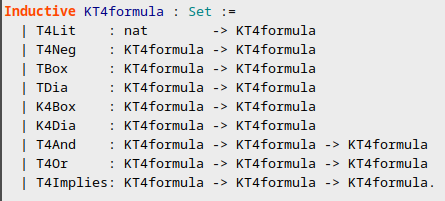
\includegraphics[scale=.6]{LinguagemKT4.png}
    %     \caption{Linguagem de \(\textbf{KT} \odot \textbf{K4}\)}
    % \end{figure}
\end{frame}
    \begin{frame}{Implementação - Definições}
    \begin{figure}[htbp]
        \centering
        % Nota: colocar aqui a função φ' e tirar ela do slide seguinte
        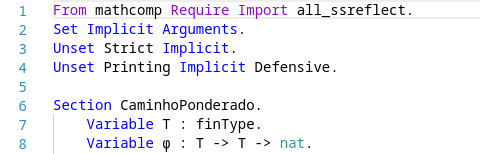
\includegraphics[scale=.6]{Definicoes1.png}
        \caption{Definições de caminhos ponderados}
    \end{figure}
\end{frame}
    \begin{frame}{Implementação - Definições}
    \begin{figure}[htbp]
        \centering
        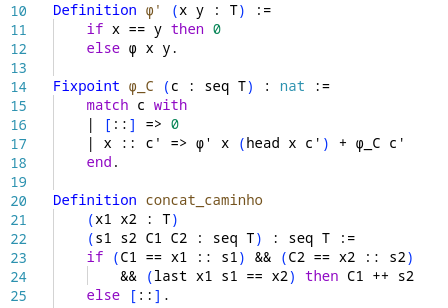
\includegraphics[scale=.6]{Definicoes2.png}
        \caption{Definições de caminhos ponderados}
    \end{figure}
\end{frame}
    \begin{frame}{Implementação - Lemas Auxiliares}
    \begin{figure}[htbp]
        \centering
        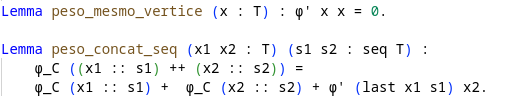
\includegraphics[scale=.6]{LemasAux.png}
        \caption{Declaração dos lemas auxiliares}
    \end{figure}
\end{frame}
    \begin{frame}{Implementação - Lemas}
    \begin{figure}[htbp]
        \centering
        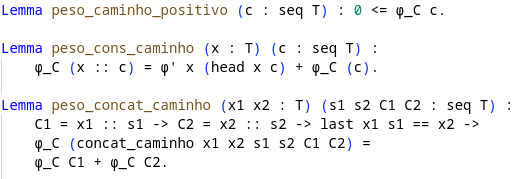
\includegraphics[scale=.6]{Lemas.png}
        \caption{Declaração dos lemas}
    \end{figure}
\end{frame}

    \section[]{Conclusões Parciais}
    \begin{frame}{Conclusões Parciais}
    \begin{itemize}
        \item A modelagem de grafos no Coq ainda está sendo estudada
        \item Resultados obtidos da implementação são positivos e indicam que é possível uma modelagem de grafos ponderados em Coq.
    \end{itemize}
\end{frame}
    \begin{frame}{Cronograma}
    \begin{enumerate}
        \item Modelar grafos ponderados no Coq;
        \item Implementar e formalizar o Algoritmo de Dijkstra;
        \item Estudar heurísticas que geram o menor caminho na Busca A*;
        \item Implementar e formalizar o Algoritmo de Busca A*.
    \end{enumerate}
\end{frame}
    \begin{frame}{Cronograma}
    \begin{table}[htpd]
        \centering
        \noindent \begin{tabular}{|c|c|c|c|c|c|c|c|}
            \hline
            \multirow{2}{*}{\textbf{\small{Etapas}}} & \multicolumn{1}{|c|}{\textbf{\small{2023/1}}} &
            \multicolumn{5}{|c|}{\textbf{\small{2023/2}}} \\
            \cline{2-7}
            &\textbf{Jul} & \textbf{Ago} & \textbf{Set} & \textbf{Out} & \textbf{Nov} & \textbf{Dez} \\
            \hline
            % \textbf{\small{1}}  & \cellcolor{gray} & \cellcolor{gray} & & & & \\
            % \hline
            \textbf{\small{1}}  & \cellcolor{gray} & \cellcolor{gray} & \cellcolor{gray} & & & \\
            \hline
            \textbf{\small{2}}  & & \cellcolor{gray} & \cellcolor{gray} & & & \\
            \hline
            \textbf{\small{3}}  & & & \cellcolor{gray} & \cellcolor{gray} & & \\
            \hline
            \textbf{\small{4}}  & & & & \cellcolor{gray} & \cellcolor{gray} & \\
            \hline
            \end{tabular}
        \label{tab:Cronograma}
        \caption[Cronograma Proposto para o TCC2]{Cronograma Proposto para o TCC2}
    \end{table}
\end{frame}

    \section[]{Referências}
    \begin{frame}[allowframebreaks]{Referências}
        \bibliography{referencias}
    \end{frame}

\end{document}